\documentclass[10pt]{article}

\usepackage{fullpage}
\usepackage{graphics}
\usepackage{natbib}
\usepackage{amssymb,amsthm,amsmath}

\newtheorem{proposition}{Proposition}
\newtheorem{lemma}[proposition]{Lemma}
\newtheorem{corollary}[proposition]{Corollary}
\newtheorem{theorem}[proposition]{Theorem}

\newcommand{\R}{\mathbb{R}}

\renewcommand{\P}{\mathcal{P}}
\newcommand{\indicator}[1]{\mathbf{1}\left[{#1}\right]}
\newcommand{\x}{\mathbf{x}}

\DeclareMathOperator{\argmin}{argmin}
\DeclareMathOperator{\err}{err}
\DeclareMathOperator{\Exp}{\mathbf{E}}
\DeclareMathOperator{\VC}{VC}

\begin{document}

\title{The information-theoretic value of unlabeled data in semi-supervised learning}
\author{Alexander Golovnev \and D\'avid P\'al \and Bal\'azs Sz\"or\'enyi}

\maketitle

\begin{abstract}
We show a separation of labeled sample complexity between learning \emph{with}
and \emph{without} the knowledge of the distribution of the unlabeled data. For
the class of projections over the boolean hypercube of dimension $n$, we show a
separation by $\Theta(\frac{\log n}{\log \log n})$ multiplicative factor.

Learning with the knowledge of the distribution (a.k.a. \emph{fixed-distribution
learning}) can be viewed as an idealized scenario of semi-supervised learning
where the number of unlabeled data points is so great that the unlabeled
distribution is known exactly. For this reason, we call the separation
the \emph{value of unlabeled data}.
\end{abstract}


\section{Introduction}

\cite{Hanneke-2016} showed that for any class $C$ of Vapnik-Chervonenkis
dimension $d$ there exists an algorithm that $\epsilon$-learns any target
function from $C$ under any domain distribution  from $O\left(\frac{d +
\log(1/\delta)}{\epsilon}\right)$ labeled examples with probability at least
$1-\delta$. \cite{Benedek-Itai-1991} showed that for any class $C$ and any
distribution there exists an algorithm that $\epsilon$-learns any target from
$C$ from $O \left( \frac{\log N + \log (1/\delta)}{\epsilon}\right)$ labeled
examples with probability at least $1-\delta$ where $N$ is the size of an
$\epsilon$-covering of $C$ with respect to the disagreement metric $d(f,g) =
\Pr[f(x) \neq g(x)]$.

Benedek-Itai's algorithm requires as input the distribution of unlabeled data in
order to construct an $\epsilon$-cover. Unsurprisingly, there exists
distributions for which Benedek-Itai's bound on the sample complexity is
significantly lower then the Hanneke's bound. For instance, a distribution with
support on a single point has cover of size $2$. That leaves the possibility
that there exists an algorithm that does \emph{not} depend on the distribution
and achieves Benedek-Itai bound (or a slightly worse bound) for \emph{every}
distribution. In fact, one would think that empirical risk minimization (ERM) or
Hanneke's algorithm could be such algorithm. (The reason one might think that is
that, for example, ERM needs only one labeled example to learn if the unlabeled
distribution is concentrated on single point.) If ERM, Hanneke's algorithm, or
some other distribution-independent algorithm had sample complexity that matches
(or nearly matches) the best known distribution-specific bound for \emph{every}
distribution, we could conclude that the knowledge of unlabeled data
distribution is completely useless.

As \cite{Darnstadt-Simon-Szorenyi-2013} showed this not the case. Any algorithm
that does not depend on the unlabeled data, requires, for some data
distributions, significantly more labeled examples than the Benedek-Itai bound.
In this paper, we quantify this gap and we show that any
distribution-independent algorithm for learning the class of projections over
$\{0,1\}^n$ requires $\Omega(\frac{\log n}{\log \log n})$ as many samples as
Benedek-Itai bound for some unlabeled distributions.

\section{Related Work}

The question of whether knowledge of unlabeled data distribution helps was
proposed and initially studied by \cite{Ben-David-Lu-Pal-2008}. However, their
paper considers only classes with Vapnik-Chervonenkis dimension at most $1$
or distributions where the size of the covering is
$\Theta(1/\epsilon)^{\Theta(\VC(C))}$ i.e. as large as it can be.\footnote{For
any concept class and any distribution, the size of the smallest
$\epsilon$-cover is at most $O(1/\epsilon)^{O(\VC(C))}$.} In these settings,
separation does not exist and they (incorrectly) concluded that unlabeled data
are useless.

The question was studied in earnest by \cite{Darnstadt-Simon-Szorenyi-2013} who
show two major results. First, they show that for any concept class $C$ and for
every distribution the ratio of the sample complexities between
distribution-independent and distribution-dependent algorithms is at most
$\VC(C)$. Second, they show that for the class of projections over $\{0,1\}^n$,
there are distributions where the ratio grows to infinity as a function of $n$.

In learning theory, the disagreement metric and $\epsilon$-cover was  introduced
by \cite{Benedek-Itai-1991} but the ideas are much older; see
e.g.~\cite{Dudley-1978, Dudley-1984}. The $O(1/\epsilon)^{O(\VC(C))}$ upper
bound on size of the smallest $\epsilon$-cover is by \citet[Lemma
7.13]{Dudley-1978}; see also \citet[Chapter 4]{Devroye-Lugosi-2000} and
\cite{Haussler-1995}.

For any distribution-independent algorithm and any class $C$ of
Vapnik-Chervonenkis dimension $d \ge 2$ and any $\epsilon \in (0,1)$ and $\delta
\in (0,1)$ there exists a distribution over the domain and a concept which
requires at least $\Omega \left(\frac{d + \log(1/\delta)}{\epsilon}\right)$
examples to $\epsilon$-learn with probability at least $1 - \delta$;
see~\cite[Theorem 5.3]{Anthony-Bartlett-1999} and
\cite{Blumer-Ehrenfeucht-Haussler-Warmuth-1989,
Ehrenfeucht-Haussler-Kearns-Valiant-1989}. The proof of the lower bound
constructs a distribution that does \emph{not} depend on the algorithm. The
distribution is a particular distribution over a fixed set shattered by $C$. So
even an algorithm that knows the distribution requires $\Omega \left(\frac{d +
\log(1/\delta)}{\epsilon}\right)$ to learn.

To better understand the relationship of the upper and lower bounds, we
summarize the situation for the class of projections over $\{0,1\}^n$ in
Figure~\ref{figure:sample-complexity}. Recall that Vapnik-Chervonenkis dimenion
of projections over $\{0,1\}^n$ is $\lfloor \log_2 n \rfloor$. This is a
folklore result, which we re-prove as
Proposition~\ref{proposition:vc-dimension-projections}.

\begin{figure}
\centering
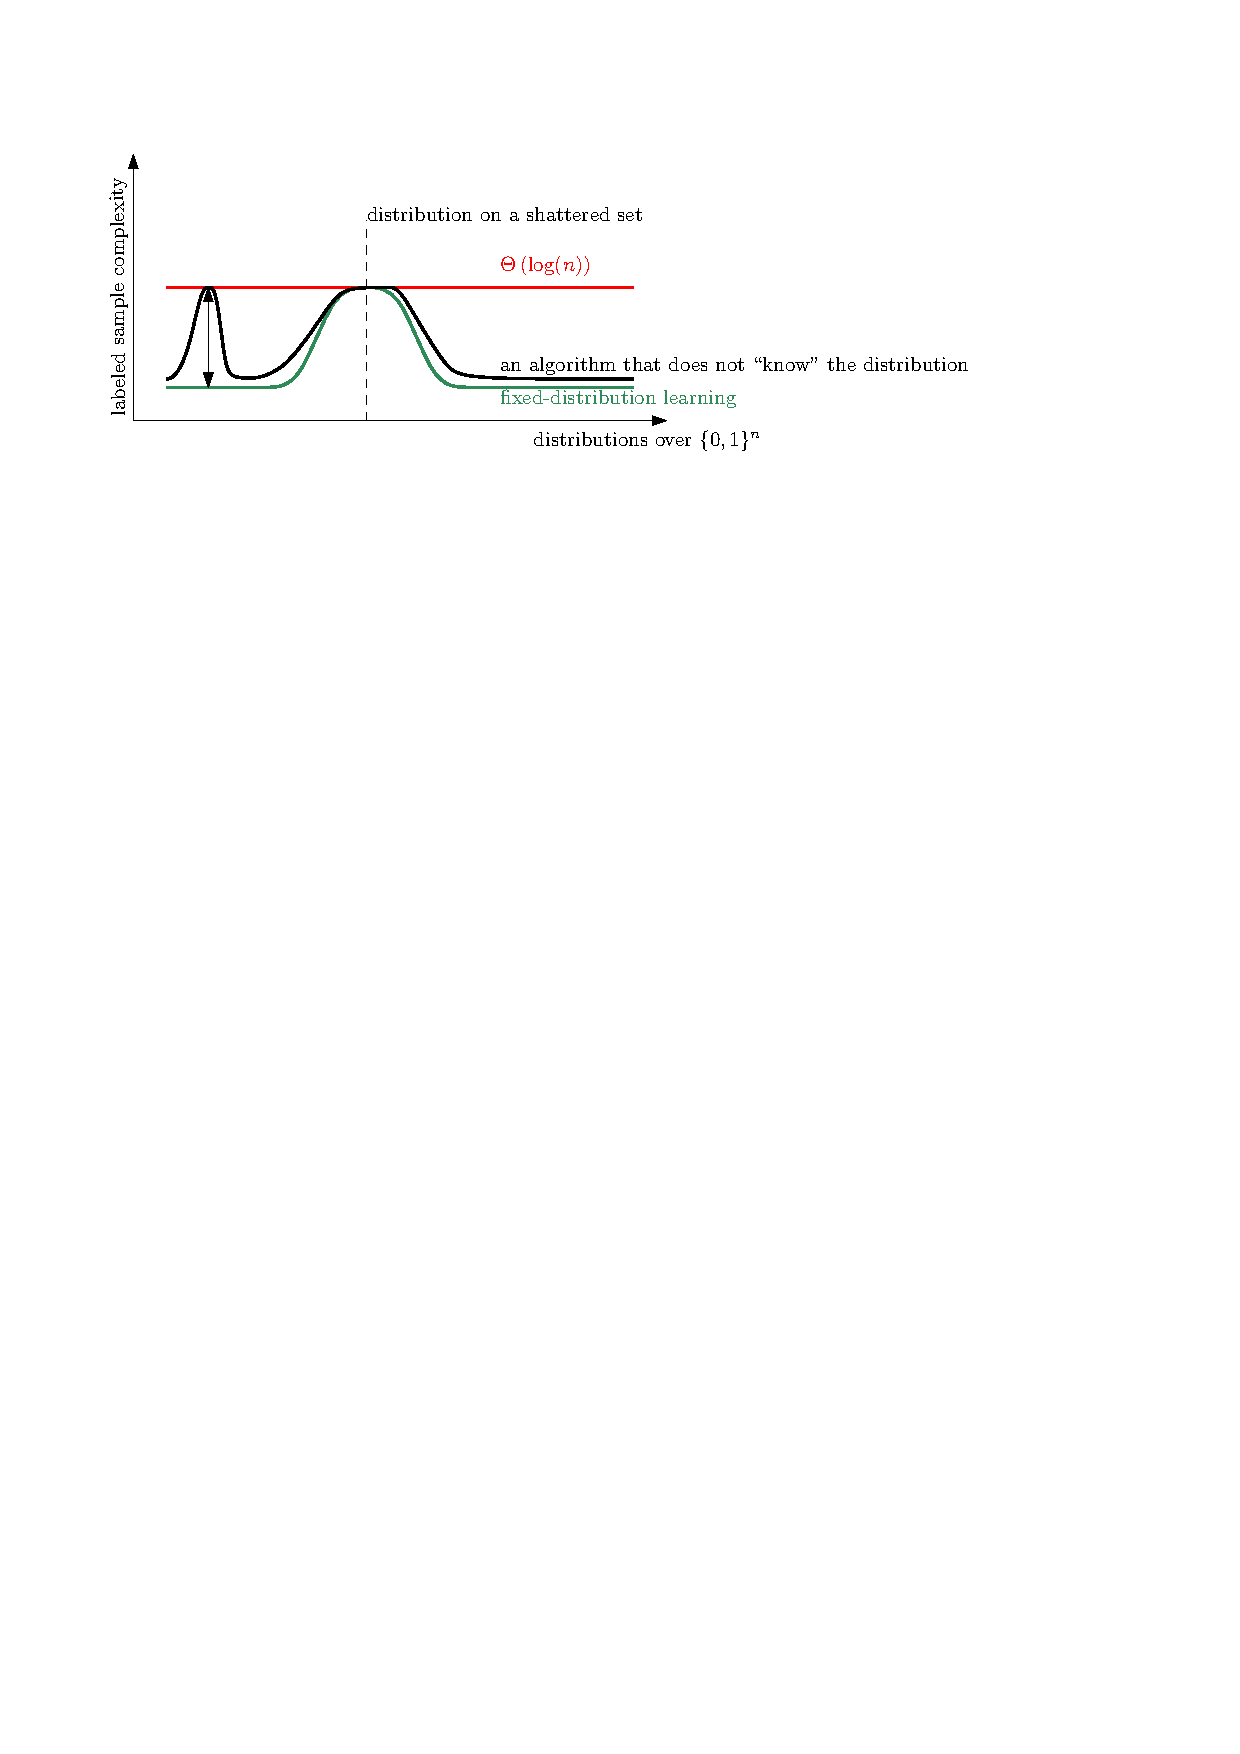
\includegraphics{figure}
\caption{The graph shows sample complexity bounds of learning a class of
projections over the domain $\{0,1\}^n$ under various unlabeled distributions.
We assume that $\epsilon$ and $\delta$ are constant, say, $\epsilon = \delta =
\frac{1}{10}$. The graph shows three lines. The red horizontal line is the
optimal Hanneke's bound for the class of projections, which is
$\Theta(\VC(C_n)) = \Theta(\log n)$. The green line corresponds to to
Benedek-Itai bound. The green line touches the red line for certain
distributions, but is lower for other distributions. In particular, for certain
distributions the green line is $O(1)$. The dashed line corresponds
to a particular distribution on a shattered set. This is where the green line
and red line touch. Futhermore, here the the upper bound coincide
with the lower bound for that particular distribution.
The black line is the sample complexity
of an arbitrary \emph{distribution-independent} algorithm. (For example, the
reader can think of the ERM or Hanneke's algorithm.) Obviously, the black line
must lie above the green line. We prove that there exist a distribution where
the black line is $\Omega(\frac{\log n}{\log \log n})$ times higher than the
green line.} \label{figure:sample-complexity}
\end{figure}

\section{Projections}

We denote by $C_n$ the class of projections over the domain $\{0,1\}^n$. The
class $C_n$ consists of $n$ functions $c_1, c_2, \dots, c_n$ from $\{0,1\}^n$ to
$\{0,1\}$. For any $i \in \{1,2,\dots,n\}$, for any $x \in \{0,1\}^n$,
the function $c_i$ is defined as $c_i((x[1], x[2], \dots, x[n])) = x[i]$.

\begin{proposition}
\label{proposition:vc-dimension-projections}
Vapnik-Chervonenkis dimension of $C_n$ is $\lfloor \log_2 n \rfloor$.
\end{proposition}

\begin{proof}
Let us denote the Vapnik-Chervonenkis dimension by $d$. Recall that $d$ is the
size of the largest shattered set. Let $S$ be any shattered set of size $d$.
Then, there must be at least $2^d$ distinct functions in $C_n$. Hence, $d \le
\log_2 |C_n| = \log_2 n$. Since $d$ is an integer, we conclude that $d \le
\lfloor \log_2 n \rfloor$.

On the other hand, we construct a shattered set of size $\lfloor \log_2 n
\rfloor$. The set will consists of points $x_1, x_2, \dots, x_{\lfloor \log_2 n
\rfloor} \in \{0,1\}^n$. For any $i \in \{1,2,\dots,\lfloor \log_2 n \rfloor\}$
and any $j \in \{0,1,2,\dots,n-1\}$, we define $x_i[j]$ to be the $i$-th bit of the
in the binary representation of the number $j$. (The bit at position $i=1$ is the
least significant bit.) It is not hard to see that for any $v \in
\{0,1\}^{\lfloor \log_2 n \rfloor}$, there exists $c \in C_n$ such that $v =
(c(x_1), c(x_2), \dots, c(x_{\lfloor \log_2 n \rfloor}))$. Indeed, given $v$,
let $k \in \{0,1,\dots,2^{\lfloor \log_2 n \rfloor} - 1\}$ be the number with
binary representation $v$, then we can take $c = c_{k+1}$.
\end{proof}

The family $\P_n$ consists of $n$ probability distributions $P_1, P_2, \dots,
P_n$ over the boolean hypercube $\{0,1\}^n$. In order to describe the
distribution $P_i$, for some $i$, let $X = (X[1], X[2], \dots, X[n])$ be a
random vector drawn from $P_i$. The distribution $\P_i$ is a product
distribution, i.e., $\Pr[X = x] = \prod_{j=1}^n \Pr[X[j] = x[j]]$ for any $x
\in \{0,1\}^n$. The marginal distributions of the coordinates are
$$
\Pr[X[j] = 1] =
\begin{cases}
\frac{1}{2} & \text{if $j = i$,} \\
\frac{1}{\ln n} & \text{if $j\neq i$.} \\
\end{cases}
$$

\begin{theorem}[Fixed distribution learning]
For any $\epsilon > 0$ and any distribution from $P \in \P_n$,
there exists an algorithm such that for any $\delta > 0$
the algorithm $\frac{1}{10}$-learns any target function
from $C_n$ using $O \left( \log(1/\delta) \right)$
labeled examples with probability at least $1 - \delta$.
\end{theorem}

\begin{proof}
The proof relies on a result of \cite{Benedek-Itai-1991} for learning under
``fixed'' distributions. If $P$ is any probability distribution on some domain,
then $d_P(f,g) = \Pr_{X \sim P}[f(X) \neq g(X)]$ is a pseudo-metric on the set of all
$\{0,1\}$-valued functions on the domain. \cite{Benedek-Itai-1991} proved that
if a $C$ class of $\{0,1\}$-functions has an $\frac{\epsilon}{2}$-cover of size
$N$, then any target from $C$ is $\epsilon$-learnable from $O
\left( \frac{\log N + \log (1/\delta)}{\epsilon}\right)$ examples
with probability at least $1-\delta$.

For our purposes we pick $\epsilon = \frac{1}{5}$. We show that for any
distribution in $\P_n$ the class $C_n$ has an $\frac{1}{10}$-cover of size $N =
2$. This will imply the lemma.

Consider distribution $P_i \in \P_n$ for some $i \in \{1,2,\dots,n\}$.
Pick any $j \in \{1,2,\dots,n\}$ such that $j \neq i$.
We claim that $C' = \{ c_i, c_j \}$ is an $\frac{1}{10}$-cover of
$C_n$. That is, we claim that for any $c \in C_n$, there exists $c' \in
C'$ such that $d_{P_{\sigma}}(c,c') \le \frac{1}{10}$.

Any $c \in C_n$ is of the form $c = c_k$. If $k \in \{i,j\}$ then, trivially, $c \in C'$ and $d_{P_i}(c,c) = 0$.
Otherwise, if  $k \not \in \{i,j\}$, let $p = \frac{1}{\ln n}$,
$$
d_{P_i}(c_j, c_k)
= \Pr_{X \sim P_i}[X_j \neq X_k] \\
= 2 p (1 - p) \\
\le 2p \\
= \frac{2}{\ln n} \\
\le \frac{1}{10} \; .
$$
The last inequality is true for all $n \ge e^{20}$.
\end{proof}

\begin{proposition}[Error probability vs. Expected error]
Let $X$ be a random variable such that $X \le 1$ with probability one.
Then, for any $\epsilon \in [0, 1)$,
$$
\Pr[X > \epsilon] \ge \frac{\Exp[X] - \epsilon}{1 - \epsilon} \; .
$$
\end{proposition}

\begin{proof}
We have
$$
\Exp[X]
\le \epsilon \cdot \Pr[X \le \epsilon] + 1 \cdot \Pr[X > \epsilon]
= \epsilon \cdot (1 - \Pr[X > \epsilon]) + \Pr[X > \epsilon] \; .  \qquad \qedhere
$$
Solving for $\Pr[X > \epsilon]$ finishes the proof.
\end{proof}

\begin{proposition}[Optimality of Bayes Predictor]
Let $\mathcal{U}$ be a finite set. Let $U,V$ be a random variables such that $U \in \mathcal{U}$ and $V \in \{0,1\}$ with probability one.
Let $f:\mathcal{U} \to \{0,1\}$ be a predictor. Then,
$$
\Pr\left[ f(U) \neq V \right]
\ge \sum_{u \in \mathcal{U}} \left( \frac{1}{2} - \left| \frac{1}{2} -  \Exp \left[V \, \middle| \, U = u\right] \right| \right) \cdot \Pr[U = u] \; .
$$
\end{proposition}

\begin{proof}
We have
$$
\Pr \left[ f(U) \neq V \right] = \sum_{u \in \mathcal{U}} \Pr \left[ f(U) \neq V \, \middle| \, U = u \right] \cdot \Pr[U = u] \; .
$$
It remains to show that
$$
\Pr\left[ f(U) \neq V \, \middle| \, U = u \right]
\ge
\frac{1}{2} - \left| \frac{1}{2} -  \Exp \left[V \, \middle| \, U = u \right] \right| \; .
$$
Since if  $U=u$, the value $f(U) = f(u)$ is fixed, and hence
\begin{align*}
\Pr\left[ f(U) \neq V \, \middle| \, U = u \right]
& \ge \min\left\{ \Pr \left[ V = 1 \, \middle| \, U = u \right], \ \Pr \left[ V = 0 \, \middle| \, U = u \right] \right\} \\
& = \min\left\{ \Exp \left[ V  \, \middle| \, U = u \right], \ 1 - \Exp \left[ V \, \middle| \, U = u \right] \right\} \\
& = \frac{1}{2} - \left| \frac{1}{2} -  \Exp \left[ V  \, \middle| \, U = u \right] \right|
\end{align*}
We used the fact that $\min\{x, 1 - x\} = \frac{1}{2} - \left| \frac{1}{2} - x \right|$ for all $x \in \R$
which can be easily verified by considering two cases: $x \ge \frac{1}{2}$ and $x < \frac{1}{2}$.
\end{proof}


\begin{theorem}[Learning without knowledge of the distribution]
For any algorithm $A$ there exists a distribution $P \in \P_n$ and a target
concept $c \in C_n$ such that the algorithm requires at least  $\Omega \left(
\frac{\log n}{\log \log n} \right)$ labeled examples to $\frac{1}{10}$-learn the
target concept with probability at least $\frac{3}{4}$.
\end{theorem}

\begin{proof}
Let $A$ be any (possibly improper) learning algorithm. We formalize it is as a function
$$
A:\bigcup_{m=0}^\infty\{0,1\}^{m \times n} \times \{0,1\})^m \to \{0,1\}^{\{0,1\}^n} \; .
$$
The algorithm receives an $m \times n$ matrix and a binary vector of length $m$.
The rows of the matrix corresponds to unlabeled examples and the vector encodes
the labels. The output of the $A$ is any function from $\{0,1\}^n \to \{0,1\}$.

For any function $h:\{0,1\}^n \to \{0,1\}$ any permutation $\sigma \in S_n$, any
projection $i \in \{1,2,\dots,n\}$, define
$$
\err_i(h) = \Pr_{X \sim P_i}[h(X) \neq c_i(X)] \; .
$$
In other words, $\err_i$ is the error of $h$ with respect to the target
$c_i$ under the distribution $P_i$.

Fix the number of examples $m$ to be any non-negative less than $\frac{\log
n}{\log \log n}$. We demostrate the existence of a pair $(P,c) \in \P_n \times
C_n$ by probabilistic method. Let $I$ be chosen uniformly at from
$\{1,2,\dots,n\}$. We will show that if we feed $A$ an i.i.d. sample of size $m$
from $P_I$ labeled according to $c_I$, with probability at least $\delta$ the
error of the algorithm is at least $\epsilon$. This will imply the existence of
the pair $(P,c)$.

Formally, let $X_1, X_2, \dots, X_m$ be an i.i.d. sample from $P_I$ and
let $Y_1 = c_I(X_1), Y_2 = c_I(X_2), \dots, Y_m = c_I(X_m)$ be the target
labels. Let $X$ be $m \times n$ matrix with entries $X_i[j]$ and let $Y = (Y_1,
Y_2, \dots, Y_m)$ be the vector of labels. The output of the algorithm is $A(X,Y)$.
We will show that
\begin{equation}
\label{equation:failure-probability}
\Pr \left[\err_I(A(X,Y)) > \frac{1}{10} \right] \ge \frac{1}{4} \; .
\end{equation}
Since $\Pr \left[\err_I(A(X,Y)) \ge \epsilon \right] = \Exp\left[ \Pr \left[\err_I(A(X,Y)) \ge \epsilon \, \middle| \, \sigma, I \right] \right]$
the inequality \eqref{equation:failure-probability} implies that there
exists $i \in \{1,2,\dots,n\}$ such that under the
distribution $P_i$, the algorithm $A$ fails to $\frac{1}{10}$-learn the target
$c_i$ with probability at least $\frac{1}{4}$.

To prove \eqref{equation:failure-probability}, we first introduce necessary
notation. For any $n \times m$ matrix $B$, let $B[1], B[2], \dots, B[n]$ be its
columns and let $c(B) = \{ j \in \{1,2,\dots, n\} ~|~ \ B[j] = B[1] \}$ be the set
of indices of columns matching the first column. Note that $1 \in c(B)$. For any
subset $K \subseteq \{1,2,\dots,n\}$, we define $p(K) = \sum_{j \in K} p_j$
where $p_j = 1/\log_2(3 + j)$. For any set $K \subseteq \{1,2,\dots,n\}$, let
$S_n(K) = \{ \pi \in S_n ~:~ \forall j \in \{1,2,\dots,n\} \setminus K, \ \pi(j) =
j \}$ be the set of permutations of $\{1,2,\dots,n\}$ that keeps the elements in
$K$ in place. There are $|K|!$ permutations in $S_n(K)$. For any permutation $\pi \in S_n$
and any $m \times n$ matrix $B$, let $\pi(B)$ an $m \times n$ matrix
$$
\pi(B) = \left[ B[\pi(1)], B[\pi(2)], \dots, B[\pi(n)] \right]
$$
with columns permuted according to $\pi$.

Let $M$ be $m \times n$ binary matrix $M = \sigma(X)$. Note that
$$
\Pr[M_{i,j} = 1] = \Pr[X_i[\sigma(j)] = 1] = p_j \qquad \qquad \text{for $i=1,2,\dots,m$, \ $j=1,2,\dots,n$}
$$
and that the entries of $M$ are independent. Also, note that $M$ and $\sigma$
are independent.

Let $\alpha$ be randomly chosen from $S_n(c(M))$. Note that $\sigma$ and
$\alpha$ are independent. Somewhat less obviously, $\alpha \circ \sigma$ and $M$
are independent and thus $(M,\sigma)$ and $(M, \alpha \circ \sigma)$ have the
same distribution; this is due to the fact that conditioned on $M$ and $\alpha$,
both $\sigma$ and $\alpha \circ \sigma$ have uniform distribution over $S_n$.

Since $X = \sigma^{-1}(M)$ and $M = \alpha(M) = \alpha^{-1}(M)$ and $Y = X[J] = X[\sigma(1)] = M[1]$,
\begin{align*}
& \Pr \left[ \err_{\sigma,J}(A(X,Y)) \ge \epsilon \right] \\
& = \Pr \left[ \err_{\sigma,\sigma(1)}(A(\sigma^{-1}(M), M[1])) \ge \epsilon \right] \\
& = \Pr \left[ \err_{\alpha \circ \sigma,\alpha(\sigma(1))}(A(\sigma^{-1} (\alpha^{-1}(M)), M[1])) \ge \epsilon \right] \\
& = \Pr \left[ \err_{\alpha \circ \sigma,\alpha(\sigma(1))}(A(\sigma^{-1}(M), M[1])) \ge \epsilon \right] \\
& \ge \Pr \left[ p(c(M)) \ge \tfrac{1}{2} + \epsilon \ \wedge \ \err_{\alpha \circ \sigma,\alpha(\sigma(1))}(A(\sigma^{-1}(M), M[1])) \ge \epsilon \right] \\
& = \sum_{\substack{\pi \in S_n \\ B \in \{0,1\}^{n \times m} \\ p(c(B)) \ge \frac{1}{2} + \epsilon}} \Pr \left[ \sigma = \pi \ \wedge \ M = B  \ \wedge \ \err_{\alpha \circ \pi,\alpha(\pi(1))}(A(\pi^{-1}(B), B[1])) \ge \epsilon \right] \\
& = \sum_{\substack{\pi \in S_n \\ B \in \{0,1\}^{n \times m} \\ p(c(B)) \ge \frac{1}{2} + \epsilon}} \Pr \left[ \err_{\alpha \circ \pi,\alpha(\pi(1))}(A(\pi^{-1}(B), B[1])) \ge \epsilon \, \middle| \, M = B \wedge \sigma = \pi \right] \cdot \Pr[M = B] \cdot \Pr[\sigma = \pi]
\end{align*}
Fix a matrix $B \in \{0,1\}^{n \times m}$ and a permutation $\pi \in S_n$. Conditioned on $M = B$ and $\sigma = \pi$,
$\alpha$ is uniformly distributed on $S_n(B)$ and $h = A(\pi^{-1}(B), B[1])$ is a fixed non-random classifier.
We compute
\begin{align*}
\Exp \left[ \err_{\alpha \circ \pi,\alpha(\pi(1))}(h) \, \middle| \, M = B \wedge \sigma = \pi \right]
& = \frac{1}{|c(B)|!} \sum_{\alpha \in S_n(B)} \err_{\alpha \circ \pi,\alpha(\pi(1))}(h) \\
& = \frac{1}{|c(B)|!} \sum_{\alpha \in S_n(B)} \Pr_{Z \sim P_{\alpha \circ \pi}} \left[ h(Z) \neq c_{\alpha(\pi(1))}(Z) \right] \\
\end{align*}

\end{proof}


\section{Monotone Disjuctions}

Consider the class $C_n$ of monotone disjuctions over $D_n = \{0,1\}^n$.
There are $2^n$ functions in $C_n$. For each subset $I \subseteq \{1,2,\dots,n\}$
there is monotone disjuction $c_I:D_n \to \{0,1\}$ defined by
$$
c_I(x) = \bigvee_{i \in I} x_i \; .
$$
We define $c_\emptyset$ to be constant zero function.

We consider the same family of distributions $\P_n$ as in the previous section.
Let $P = P_{Identity} \in \P_n$. We compute the distance $d_P(c_I, c_J)$
between any two monotone disjuctions. For any subset
$K \subseteq \{1,2,\dots,n\}$, let $A_K$ be the event that all for all $i \in K$, $x_i = 0$.
\begin{align*}
d_P(c_I, c_J)
& = \Pr_{x \sim P}[c_I(x) \neq c_J(x)] \\
& = \Pr_{x \sim P}[A_{I \cap J} \wedge ((A_{I \setminus J} \wedge \overline{A_{J \setminus I}}) \vee (\overline{A_{I \setminus J}} \wedge A_{J \setminus I} )) ] \\
& = \Pr[A_{I \cap J}] \cdot \left\{ \Pr[A_{I \setminus J}] (1 - \Pr[A_{J \setminus I}]) + (1 - \Pr[A_{I \setminus J}]) \Pr[A_{J \setminus I}] \right\} \\
& = \Pr[A_{I \cap J}] \cdot \left\{ \Pr[A_{I \setminus J}] + \Pr[A_{J \setminus I}] - 2 \Pr[A_{I \setminus J}] \Pr[A_{J \setminus I}] \right\} \\
& = \Pr[A_I] + \Pr[A_J] - 2 \Pr[A_{I \cup J}] \\
& = \prod_{i \in I} (1 - p_i) + \prod_{j \in J} (1 - p_j) - 2 \prod_{k \in I \cup J} (1 - p_k) \; . \\
\end{align*}

\bibliography{biblio}
\bibliographystyle{plainnat}

\end{document}
